\chapter{Clustering Methods} \label{ch:clusteringMethods}
So far we have looked only at supervised learning, where a correct pair of input and output variables ($X$ and $y$) were given to train the model and verify our results. An analog to this is a teacher supervising the learning. The teacher have the correct answers and the algorithm iteratively makes predictions on our data and is corrected by the teacher. In unsupervised learning we do not have a output variable $y$, only the features $X_1$, $X_2$,...,$X_p$. This compel us to not look at predictions, but rather interesting things about the observed measurements and possibly discover subgroups in the data. We use clustering as a technique to perform unsupervised learning. In this chapter we will look at K-means and hierarchical clustering.

\section{K-means Clustering}
\subsection{Theory}
The way that K-means clustering works is that there is a $C_1,...,C_k$ sets that contains part of the observations. These sets needs to satisfy two properties.
\begin{enumerate}
	\item $ C_1 \cup C_2 \cup ... \cup C_K = \{ 1,...,n \}$ Which means each observation belongs to at least one of the K clusters.
	\item $ C_k \cap C_{k'} = \emptyset $ for all $k \neq k'$ Which means the clusters are non-overlapping basically no observation belongs to more then one cluster.
\end{enumerate}

The goal of K-means clustering is to find good clusters with as small as possible within-cluster-variation. The Equation \ref{fo:k-meansMini}, tries to partition the observations into K clusters to achieve this.
\begin{align}\label{fo:k-meansMini}
\sum_{k=1}^{k} WCV(C_K)
\end{align}
To do this we need a distance metric. The one that is typically used is Euclidean distance, given by $d = \sqrt{ (x_2 - x_1)^2 - (y_2 - y_1)^2 } $. Which means the distance between two points is the length of the path connecting them or in other words the straight-line distance between two points in a plane. In Equation \ref{fo:EuclideanDistance1} $ |C_k| $ represent the number of observations in the \textit{k}'th cluster.
\begin{align}\label{fo:EuclideanDistance1}
WCV(C_K) = \dfrac{1}{|C_k|}  \sum_{i,i' \in C_k}   \sum_{j=1}^{p}(x_ij - x_{i'}j)^2
\end{align}
If we combine our two formulas given in \ref{fo:k-meansMini} and \ref{fo:EuclideanDistance2} we will get a optimization problem that defines K-means clustering. Were we try to minimize $ C_1,...,C_k $.
\begin{align}\label{fo:EuclideanDistance2}
\sum_{k=1}^{k} \dfrac{1}{|C_k|}  \sum_{i,i' \in C_k}   \sum_{j=1}^{p}(x_ij - x_i'j)^2
\end{align}

The K-Means Clustering Algorithm works like this
\begin{enumerate}
	\item The k centroids are placed at random.
	\item Assign each observation to the nearest of the k clusters.
	\item Move the centroids to the center of their clusters. The new position of each centroid is calculated as the average position of all the points in its cluster.
\end{enumerate}
We keep repeating steps 2 and 3 until the algorithm converges( centroid stop moving a lot at each iteration ).

\subsection{Results} %TODO rewrite (remove code etc.)
\subsubsection*{LAB 10.5.1}
Lab 10.5.1 is using the k-means clustering to group data. The lab begins by making a normal distribution put into a 25x2 matrix and in which there are two clusters in the data. Then changing the first 25 observations with a mean shift relative to the next 25 observations.

Then running the K-means clustering with K = 2 and 20 iterations. As it can be seen output of the algorithm is a set of labels assigning each observation to one of the k groups. The way that these groups are made is by creating a centroid for each group. The centroids are the middle of the cluster and they capture the points closest to them and adds them to the cluster. The plot of this can be seen in figure \ref{fig:kmeansclusteringk2_20Iteration} on the right.

Next we run the K-means clustering with K = 3 and 20 iterations. The plot of this can be seen in figure \ref{fig:kmeansclusteringk2_20Iteration} on the left.

\begin{figure}[H]
	\centering
	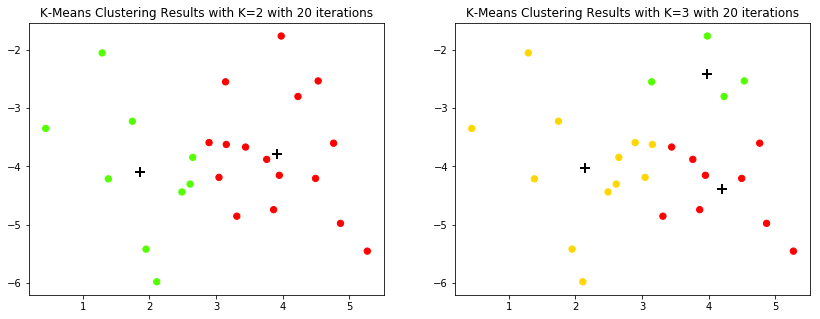
\includegraphics[width=0.7\textwidth]{clusteringMethods/kmeansclustering/fig/k-mean.png}
	\caption{K-Means Clustering Results with K=2 with 20 iterations on the right and  with K=3 with 20 iterations on the left}
	\label{fig:kmeansclusteringk2_20Iteration}
\end{figure}

While k-means clustering is a good algorithm, it is not without it's own flaws. When running K-means clustering with a large number of iterations, such as 20 since otherwise an undesirable local optimum may be obtained. Which simply means that, more than one run of the algorithm with randomized starting centroids could give a better result.




\section{Hierarchical clustering}

With K-means clustering we had to predefine the number of clusters $K$. This can be a disadvantage, since we would have to do some initial analysis of the data prior to clustering it. Hierarchical clustering does not require this predefinition. It uses a bottom-up tree algorithm or agglomerative approach to build a dendrogram starting from the observation leaves and ends up combining this into clusters at the trunk. This gives us a flexibility in the number of clusters.

\subsection{Theory}

Agglomerative states that each observation starts in its own cluster and with each iteration of the process are paired with other clusters as we move up the hierarchy.  This is based on a \textit{metric} criteria, a measure of distance between the pairs, and a \textit{linkage} criteria that indicate the dissimilarity between pairwise sets.

A common metric is the Euclidean distance:
\begin{align}
	d(a,b) = \sqrt{\sum (a_{i} - b_{i})^{2}}  %TODO Christian did you done goof in equation 7.4? with the underlined 2
\end{align}

Which is the straight-line distance between two points in Euclidean space (\textit{n}-space with \textit{n}-tuples of real numbers). Between two points \textit{a} and \textit{b} given by ($X_a$, $Y_a$) and ($X_b$, $Y_b$) the Euclidean distance d(a,b) is:
\begin{align}
	d(a,b) = \sqrt{(X_a - X_b)^2 + (Y_a - Y_b)^2}
\end{align}

Linkage determines which distances to use between sets of observations, i.e. how they are grouped together. \textit{Single} minimizes the distance between the closest elements in clusters, \textit{complete} maximizes distance between the farthest elements, \textit{average} finds the mean of all pairwise distances, and \textit{ward} joins clusters based on the total distance between their centroids. Figure \ref{fig:linkagecriteria} shows the three kinds of linkages to calculate distance.

\begin{figure}[H]
	\centering
	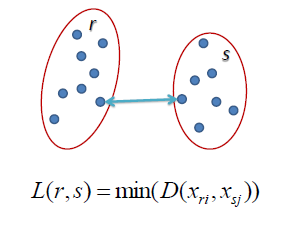
\includegraphics[width=0.3\textwidth]{clusteringMethods/hierarchicalclustering/fig/ClusteringSingle.png}
	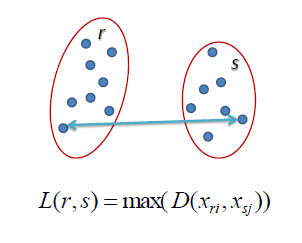
\includegraphics[width=0.3\textwidth]{clusteringMethods/hierarchicalclustering/fig/ClusteringComplete.png}
	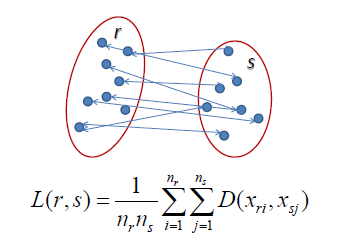
\includegraphics[width=0.3\textwidth]{clusteringMethods/hierarchicalclustering/fig/ClusteringAverage.png}
	\caption{The single, complete and average linkage criteria.}
	\label{fig:linkagecriteria}
\end{figure}

The algorithmic steps for hierarchical clustering are:

1. Start with \textit{N} clusters, one for each data point. \\
2. Merge the clusters that are closest to each other. This gives \textit{N-1} clusters. \\
3. Calculate the distance between the clusters using a linkage criteria (complete, single etc.) \\
4. Repeat step 2 and 3 until we end up with one cluster with \textit{N} data points. The end result is a dendrogram picturing the distance (clusters) as a function of the observations (labels).

\subsection{Results}
\subsubsection*{LAB 10.5.2}%TODO rewise exercise
Lab 10.5.2 is using hierarchical clustering to group a 50 x 50 matrix of random observations using Euclidean distance and complete linkage in to two clusters. The AgglomerativeClustering package from Sklearn provides agglomerative clustering functionality in Python to recursively merge pairs of clusters.The Agglomerative Clustering gives the following output.

\noindent\textit{Labels:[1 0 1 1 0 0 0 0 0 0 1 0 0 0 1 0 0 1 10]}

\noindent\textit{No. leaves:  20}

\noindent\textit{No. clusters:  2}


\noindent labels from the complete agglomerative clustering process show how the observations are grouped, starting from $X_i$ to $X_n$. A label [0 1 1 1 0] says observation $X_0$ belongs to the first final cluster, $X_1$ to the second final cluster, $X_2$ to the second etc. The number of leaves correspond to the observations points ($X_a$, $Y_a$). We then generate a dendrogram to picture the Euclidean distance between clusters and their labels. Figure \ref{fig:dendrogramcluster} shows the dendrograms of the three performed clusterings.

\begin{figure}[H]
	\centering
	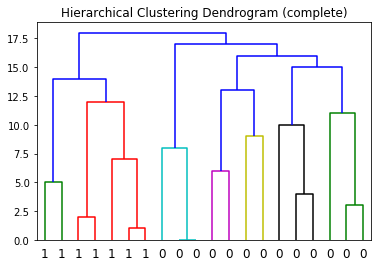
\includegraphics[width=0.3\textwidth]{clusteringMethods/hierarchicalclustering/fig/CompleteClustering.png}
	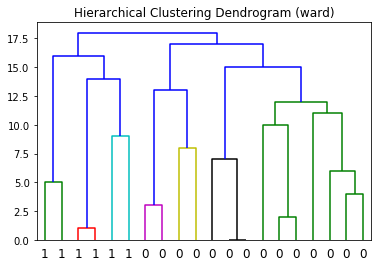
\includegraphics[width=0.3\textwidth]{clusteringMethods/hierarchicalclustering/fig/WardClustering.png}
	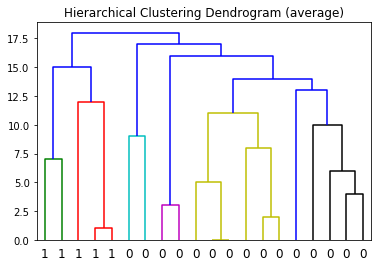
\includegraphics[width=0.3\textwidth]{clusteringMethods/hierarchicalclustering/fig/AverageClustering.png}
	\caption{Dendrograms for complete, ward and average clustering.}
	\label{fig:dendrogramcluster}
\end{figure}

\noindent Also in Figure \ref{fig:dendrogramcluster} is sowing that hierarchical clustering correctly identifies the lower left cluster and the lower right one, however with ward and average a significant euclidean distance has to be reached for it to split correctly, whereas complete splits the observations into two separate ones early on. 

%TODO What is a ward Christian?








